\documentclass[12pt,a4paper]{report}
\usepackage{graphicx}
\usepackage{amsmath}
\usepackage{fancyhdr}
\usepackage{cite}
\usepackage{framed}
\usepackage{a4wide}
\usepackage{float}
\usepackage{epsfig}
\usepackage{longtable}
\usepackage{enumerate}
\usepackage{afterpage}
\usepackage{multirow}
\usepackage{ragged2e}
\usepackage{gensymb}
\usepackage{amsfonts} 
\usepackage[left=3.5cm,top=1.5cm,right=3cm,bottom=4cm]{geometry}
\usepackage{setspace}           
\usepackage{txfonts}
\usepackage{lipsum}

\newcommand{\Usefont}[1]{\fontfamily{#1}\selectfont}

\usepackage{lscape}
\renewcommand{\baselinestretch}{1.7} 

\usepackage{blindtext}
\usepackage{xpatch}
\usepackage{url}
\usepackage{leqno}
\usepackage{subcaption}
\usepackage{booktabs}

\linespread{1.5}
\usepackage[intoc, english]{nomencl}
\hyphenpenalty=5000
\tolerance=1000
\usepackage[nottoc]{tocbibind}

% References config
\bibliographystyle{IEEEtran}
\renewcommand{\bibname}{References}

\graphicspath{{figures/}}

\begin{document}
	
% Global Definitions
\gdef \title{An Independence Platform for Voice-Native OS Navigation by Individuals with Severe Motor Impairment}
\gdef \dept{Computer Science and Engineering}
\gdef \degree{Bachelor of Technology}
\gdef \branch{Computer Science and Engineering}
\gdef \college{SCT College of Engineering}
\gdef \collegeplace{Thiruvananthapuram}
\gdef \studentA{Abhiram A. R.}
\gdef \studentAroll{SCT23CS007}
\gdef \studentB{Kevin L.}
\gdef \studentBroll{SCT23CS037}
\gdef \studentC{Niyatha Suresh R.}
\gdef \studentCroll{SCT23CS051}

\gdef \guide{Prof. Dr. Subu Surendran}
\gdef \guidedes{Professor}

\gdef \projadvisor{Asst. Prof. Binu Rajan M. R.}
\gdef \projadvisordes{Assistant Professor}

\gdef \hod{Assoc. Prof. Rejimol Robinson R. R.}
\gdef \hoddes{Associate Professor and Head}

\gdef \acadyear{2025 - 2026}
\gdef \month{October 2026}
\gdef \date{29-10-2026}

% Front pages
%==================================coverpage.tex================================

\thispagestyle{empty}
\begin{titlepage}
	\begin{center}
		{\Usefont{phv} \Large \bf \title \par}
		\vspace*{30pt}
		\large \em \Usefont{pzc}{ 
			A Project Report \par
			Submitted to the APJ Abdul Kalam Technological University\\
			in partial fulfillment of requirements for the award of degree}\\ [.15\baselineskip] \par
		\vspace*{10pt}
		\Usefont{ppl} {\bfseries  \degree}\\
		in\\
		{\Usefont{ppl} {\bfseries \branch}}\\
		\vspace*{15pt}
		by\\
		\vspace*{10pt}
		\bf {\studentA}\hspace*{5pt}(\studentAroll)\\
		\bf {\studentB}\hspace*{5pt}(\studentBroll)\\
		\bf {\studentC}\hspace*{5pt}(\studentCroll)\\
		\vspace*{25pt}
		\centering
		\begin{figure}[h!]
			\centerline{
\includegraphics[scale=0.6]{cet_logo}}
		\end{figure}
		
		\vspace{\stretch{0.5}}
		\footnotesize{\bf DEPARTMENT OF COMPUTER SCIENCE AND ENGINEERING} \par
		\bf{SCT COLLEGE OF ENGINEERING} \par
		\bf{THIRUVANANTHAPURAM, KERALA} \par
		\bf{\month}
	\end{center}		
\end{titlepage}

%==================================certificate1.tex================================
% Certificate page with Guide, Project Advisor, and Head of Department

\newpage
\begin{center}	
	\textbf{DEPARTMENT OF COMPUTER SCIENCE \& ENGINEERING}	\\
	\textbf{SCT COLLEGE OF ENGINEERING}	\\
	\textbf{THIRUVANANTHAPURAM} \\
	\vspace*{5pt}
	\textbf{\acadyear} 
\end{center}

\begin{center}
	
\includegraphics[scale=0.5]{cet_logo}	
\end{center}
\begin{center}
	\textbf{CERTIFICATE}
\end{center}

This is to certify that the report entitled \textbf{\title} submitted by \textbf{\studentA}\hspace*{2pt}(\studentAroll),\hspace*{2pt}\textbf{\studentB}\hspace*{2pt}(\studentBroll) and \textbf{\studentC}\hspace*{2pt}(\studentCroll) to the APJ Abdul Kalam Technological University in partial fulfillment of the B.Tech.\ degree in \branch \hspace*{2pt} is a bonafide record of the project work carried out by them under our guidance and supervision. This report in any form has not been submitted to any other University or Institute for any purpose.

\begin{singlespace}
	\vspace*{1.5cm}
	\begin{table}[h!]
		\centering
		\begin{tabular}{p{7cm} p{0.5cm} p{7.5cm}} 
			\textbf{\guide} && \textbf{\projadvisor} \\
			(Project Guide) &&  (Project Advisor)\\
			\guidedes & & \projadvisordes\\ 
			Dept. of CSE && Dept. of CSE\\ 
			SCT College of Engineering & & SCT College of Engineering\\
			Thiruvananthapuram && Thiruvananthapuram\\
		\end{tabular}
	\end{table}
	
	\vspace*{1.0cm}
	
	\begin{center}
		\textbf{\hod} \\ 
		\hoddes\\ 
		Dept. of CSE\\ 
		SCT College of Engineering\\
		Thiruvananthapuram\\
	\end{center}
\end{singlespace}

\thispagestyle{empty}

%==================================declaration.tex================================
%
\newpage
\thispagestyle{empty}
\begin{center}
\vspace*{30pt}
\textbf{\large DECLARATION}\\
\end{center}
\vspace*{15pt}
We hereby declare that the project report entitled {\bf{\title}}, submitted for partial fulfillment of the requirements for the award of degree of Bachelor of Technology in \branch \hspace*{2pt} of the APJ Abdul Kalam Technological University, Kerala, is a bonafide work done by us under the supervision of \textbf{\guide}, Professor, Department of Computer Science and Engineering, SCT College of Engineering, Thiruvananthapuram. \par
This submission represents our ideas in our own words and where ideas or words of others have been included, we have adequately and accurately cited and referenced the original sources.\par 
We also declare that we have adhered to ethics of academic honesty and integrity and have not misrepresented or fabricated any data or idea or fact or source in our submission. We understand that any violation of the above will be a cause for disciplinary action by the institute and/or the University and can also evoke penal action from the sources which have thus not been properly cited or from whom proper permission has not been obtained. This report has not been previously formed the basis for the award of any degree, diploma or similar title of any other University or Institution.

\vspace*{2cm}
\noindent \begin{minipage}{0.45\linewidth}
\begin{flushleft}
\collegeplace \\
\date
\end{flushleft} 
\end{minipage}
\hfill
\begin{minipage}{0.45\linewidth}
\begin{flushright}                                      
\textbf{\studentA}\\
\textbf{\studentB}\\
\textbf{\studentC}\\
\end{flushright} 
\end{minipage}
\thispagestyle{empty}


\pagenumbering{roman} 

%============================= abstract.tex================================
\chapter*{Abstract}%
\addcontentsline{toc}{chapter}{Abstract}%

Individuals suffering from severe motor impairment or full paralysis who retain speech capabilities lack adequate, accessible computational tools to independently operate a personal computer. Existing voice-based assistive solutions are fundamentally limited: traditional systems rely on brittle, predefined command-and-control grammars incapable of handling complex or unstructured intent, while emerging autonomous agent frameworks are predominantly constrained to sandboxed browser automation rather than system-wide operating system (OS) control. Furthermore, conventional voice assistants implement cascaded Speech-to-Text (STT) $\rightarrow$ Large Language Model (LLM) $\rightarrow$ Text-to-Speech (TTS) pipelines that introduce compounded round-trip latency, rely heavily on proprietary cloud connectivity, and cater almost exclusively to English-language speakers.

This project proposes an independent, voice-native, self-correcting OS navigation platform specifically engineered for individuals with severe physical disabilities. Operating at the full desktop OS level, the proposed platform harnesses a lightweight local Large Language Model (Qwen 1.5B running via a quantized \texttt{llama.cpp} runtime) orchestrated with native OS accessibility APIs and a dynamic Tool Registry. Natural, unstructured vocal instructions are converted into structured tool invocations and verified script actions covering navigation, window management, system configuration, and file manipulation. To close the perception--action feedback loop without demanding physical intervention from the user, the agent integrates a multi-modal screen-state perception module that reads the accessibility tree and visual screen state, compares expected outcomes with post-execution observations, and automatically triggers self-correction routines upon failure. 

To overcome latency and privacy bottlenecks, the platform implements a dual-mode hybrid architecture supporting fully offline local execution with an average query inference time of $\le 15$ seconds, alongside cloud model-switching capabilities that incorporate domestic Indian foundational models (such as Sarvam AI) to enable seamless regional language interaction. Additionally, an intelligent caching layer stores recurring workflows, dramatically accelerating routine operations. The system is extended via the Model Context Protocol (MCP) to seamlessly interface with modern productivity suites and developer environments. Experimental evaluation across diverse system tasks demonstrates that the proposed architecture provides a robust, low-latency, and hands-free computing environment that restores functional independence and digital productivity to paralyzed users.

\thispagestyle{plain}
%=======================================================================

%==================================acknowledgement.tex=============================
\chapter*{Acknowledgement}%
\addcontentsline{toc}{chapter}{Acknowledgement}%

\par We take this opportunity to express our deepest sense of gratitude and sincere thanks to everyone who helped us to complete this project work successfully. 

We express our profound gratitude to \textbf{\hod}, \hoddes, \dept, \college, Thiruvananthapuram, for providing us with all the necessary infrastructural facilities, continuous encouragement, and institutional support throughout the course of this project.

We extend our sincere thanks and heartfelt gratitude to our Project Advisor, \textbf{\projadvisor}, \projadvisordes, \dept, \college, for his insightful guidance, critical suggestions, and constant supervision during every phase of this project.

We place on record our earnest gratitude to our Project Guide, \textbf{\guide}, \guidedes, \dept, \college, for his invaluable mentorship, constructive feedback, technical insights, and consistent encouragement which served as an enduring source of inspiration throughout this research and implementation.

We also thank all the teaching and non-teaching staff members of the Department of Computer Science and Engineering for their direct and indirect assistance. Finally, we express our heartfelt thanks to our families and friends whose unwavering moral support, patience, and encouragement made the successful completion of this project report possible.

\vspace*{40pt}
\begin{flushright}
	\textbf{\studentA}\\
	\textbf{\studentB}\\
	\textbf{\studentC}\\
\end{flushright}
\thispagestyle{plain}


\thispagestyle{empty}
\newpage
    
% Table of Contents and Lists
\tableofcontents
\listoffigures
\listoftables
%==================================symbols.tex================================
% List of Abbreviations and Symbols
\chapter*{List of Abbreviations}
\addcontentsline{toc}{chapter}{List of Abbreviations}%

\begin{singlespace}
\begin{longtable}{p{2.5cm} p{11.5cm}}
\textbf{API} & Application Programming Interface \\
\textbf{ASR} & Automatic Speech Recognition \\
\textbf{CER} & Character Error Rate \\
\textbf{CLI} & Command-Line Interface \\
\textbf{CPU} & Central Processing Unit \\
\textbf{DAG} & Directed Acyclic Graph \\
\textbf{E2E} & End-to-End \\
\textbf{GPU} & Graphics Processing Unit \\
\textbf{HOD} & Head of Department \\
\textbf{IO} & Input / Output \\
\textbf{JSON} & JavaScript Object Notation \\
\textbf{KTU} & APJ Abdul Kalam Technological University \\
\textbf{LLM} & Large Language Model \\
\textbf{LSA} & Latent Semantic Analysis \\
\textbf{MCP} & Model Context Protocol \\
\textbf{MVP} & Minimum Viable Product \\
\textbf{NLP} & Natural Language Processing \\
\textbf{NLU} & Natural Language Understanding \\
\textbf{OS} & Operating System \\
\textbf{RAG} & Retrieval-Augmented Generation \\
\textbf{SCTCE} & Sree Chitra Thirunal College of Engineering \\
\textbf{STT} & Speech-to-Text \\
\textbf{TTS} & Text-to-Speech \\
\textbf{UI} & User Interface \\
\textbf{UIA} & Microsoft UI Automation \\
\textbf{VAD} & Voice Activity Detection \\
\textbf{Vosk} & Offline Speech Recognition Toolkit \\
\textbf{WER} & Word Error Rate \\
\end{longtable}
\end{singlespace}


% Body of the report
\cleardoublepage
\setcounter{page}{1}
\pagenumbering{arabic}

%%********************Chapter 1**********
\chapter{Introduction}
\label{chap:intro}

\section{Overview and Background}
Modern personal computing environments are fundamentally predicated on tactile manual input mechanisms, primarily the mechanical keyboard, mouse, and tactile touchscreens. For individuals afflicted with severe motor impairments, including quadriplegia, advanced cerebral palsy, amyotrophic lateral sclerosis (ALS), spinal cord trauma, or severe stroke, these conventional physical input modalities present insurmountable barriers to digital independence. Consequently, paralyzed individuals who retain fluent or partial speech capabilities must rely on assistive technologies to access computational environments for education, communication, and occupational productivity.

Voice-driven computing has emerged as the most natural, non-invasive interface for hands-free computer control. In an ideal assistive ecosystem, a voice assistant acts as an autonomous digital proxy that continuously executes a perception--action cycle: listening to spoken dialogue, synthesizing contextual intent, translating that intent into precise system commands, and executing actions directly within the native operating system (OS). Rather than functioning as a conversational passive chatbot that simply returns synthesized text, an effective accessibility agent must execute granular, reliable operations across diverse desktop software suites.

\section{Motivation and Existing Challenges}
Despite significant advancements in artificial intelligence and voice processing, current assistive software suffers from severe structural deficiencies:
\begin{enumerate}[(i)]
    \item \textbf{Rigid Command Grammars:} Traditional accessibility systems rely heavily on hardcoded rule engines and keyword dictionaries. Users are forced to memorize synthetic, non-intuitive syntaxes (e.g., ``press Control Alt T''). Any natural conversational variance, disfluency, or complex syntactic structure results in complete recognition failure.
    \item \textbf{Sandboxed Browser Limitation:} Contemporary autonomous UI agents (such as web-scraping agents) operate predominantly inside browser DOMs. They lack direct hooks into native desktop processes, legacy Win32/X11 controls, system file trees, and local desktop software suites.
    \item \textbf{High Latency of Cascaded Architectures:} Mainstream commercial voice pipelines deploy a cascaded sequence consisting of Speech-to-Text (STT) $\rightarrow$ Large Language Model (LLM) reasoning $\rightarrow$ Text-to-Speech (TTS) synthesis. In cloud deployments, network transport and serialization latencies compound across each stage, resulting in response delays exceeding several seconds, which is intolerable for real-time interactive tasks.
    \item \textbf{Absence of Verification and Self-Correction:} Existing voice navigation tools blindly dispatch synthetic keyboard or mouse events without perceptual feedback. If a window fails to gain focus or a network dialog interrupts the workflow, the system continues executing actions into an invalid state. Paralyzed users cannot physically reach a mouse or keyboard to abort erroneous operations.
    \item \textbf{Internet Dependency and Language Barriers:} Most cloud-dependent assistive agents transmit proprietary audio and screen captures to remote servers, raising critical privacy concerns. Furthermore, these platforms predominantly cater to English, effectively disenfranchising speakers of regional Indian languages.
\end{enumerate}

\section{Problem Statement}
The objective of this research is to design and implement an independent, voice-native, and self-correcting operating system navigation platform that enables individuals with severe physical and motor impairments to achieve real-time, autonomous, and productive control over personal computers without requiring physical input, sandboxed browser constraints, or continuous internet connectivity.

\section{Project Objectives}
The specific technical objectives of this project are formulated as follows:
\begin{enumerate}[1.]
    \item \textbf{Modular Agent Package:} To develop an extensible agent runtime that executes desktop navigation, system configuration, and file manipulation via native OS APIs and accessibility UI hierarchies.
    \item \textbf{Lightweight Streaming Audio Package:} To construct a low-latency, CPU-friendly speech recognition module that reliably converts natural spoken instructions into structured text on commodity hardware.
    \item \textbf{Personal Context Manager (``Second Brain''):} To design a multi-tiered context engine that captures personal user preferences, workspace profiles, visual screen history, and short-term dialogue context, resolving implicit or relative spoken commands.
    \item \textbf{Productivity Integration via Model Context Protocol (MCP):} To integrate desktop productivity plugins through the standardized Model Context Protocol, connecting the agent seamlessly with external applications such as Antigravity, Claude, PowerPoint, Word, and Canva.
    \item \textbf{Dual-Mode Hybrid Execution with Model Switching:} To support both completely offline execution (via quantized local LLMs like Qwen 1.5B) maintaining an inference threshold of $\le 15$ seconds, and cloud switching to regional Indian foundational models (such as Sarvam AI).
    \item \textbf{Intelligent Workflow Caching:} To implement a semantic caching framework for repetitive desktop workflows, drastically reducing latency and computational overhead on frequent operations.
\end{enumerate}

\section{Organization of the Report}
The remainder of this report is organized as follows:
\begin{itemize}
    \item \textbf{Chapter 2 (Literature Survey):} Presents an exhaustive literature review of contemporary research in embedded voice assistants, scalable speech recognition, and intent extraction, detailing the technical gaps that motivate this system.
    \item \textbf{Chapter 3 (System Architecture and Design):} Expounds the detailed architectural design of the platform, including the Audio Package, Agent Package, Tool Registry, Context Manager, and execution flow.
    \item \textbf{Chapter 4 (Methodology and Implementation Plan):} Outlines the modular development phases, model selection strategy, testing benchmarks, and audio evaluation protocols.
    \item \textbf{Chapter 5 (Results and Discussion):} Analyzes experimental findings, inference latencies, command execution accuracies, and comparative benchmarks against existing voice control paradigms.
    \item \textbf{Chapter 6 (Conclusion and Future Scope):} Summarizes the core contributions and discusses avenues for future research, including dysarthric speech adaptation and multimodal perception models.
\end{itemize}


%%********************Chapter 2**********
\chapter{Literature Survey}
\label{chap:lit_review}

\section{Introduction}
Developing a voice-native OS navigation system requires synthesizing research across automatic speech recognition (ASR), natural language understanding (NLU), desktop automation, and assistive computing. This chapter reviews three seminal foundational works that address embedded speech processing, high-throughput real-time ASR, and intent recognition pipelines, highlighting their critical contributions, architectural limitations, and the specific research gaps addressed by our platform.

\section{Review of Foundational Literature}

\subsection{Embedded End-to-End Voice Assistants}
Lazzaroni et al. \cite{lazzaroni2024embedded} designed and evaluated an embedded end-to-end voice assistant architecture deployed directly on localized edge hardware for intelligent vehicular and smart home environments. Their work tackled the acute privacy vulnerabilities and latency unpredictability associated with commercial cloud assistants (e.g., Amazon Alexa, Google Assistant). 

The authors developed a five-phase modular methodology:
\begin{enumerate}
    \item \textit{Phase 1 (Speech Classification):} Utilizing lightweight convolutional networks to detect acoustic wake words and filter background noise.
    \item \textit{Phase 2 (Speech Recognition):} Fine-tuning a QuartzNet 15x5 acoustic model via transfer learning to perform offline Italian ASR with competitive Word Error Rate (WER) and Character Error Rate (CER).
    \item \textit{Phase 3 (Language Understanding):} Utilizing intent-slot matching through small-scale discriminative classifiers to map text to predefined JSON actions.
    \item \textit{Phase 4 (Speech Synthesis):} Deploying lightweight embedded TTS synthesizers for acoustic confirmation.
    \item \textit{Phase 5 (System Deployment):} Deploying the quantized pipeline on embedded Nvidia Jetson and Raspberry Pi hardware without internet connectivity.
\end{enumerate}
While their system demonstrated that offline edge execution can achieve competitive ASR latency and accuracy, it relied on rigid rule templates and completely omitted generative Large Language Models due to edge memory constraints. Consequently, the assistant is incapable of handling unstructured spoken commands, multi-step desktop workflows, or dynamic error recovery.

\subsection{Scalable Real-Time Automatic Speech Recognition at Scale}
Bruzzone et al. \cite{bruzzone2026sink} investigated the architectural bottlenecks of real-time ASR under multi-stream, concurrent user workloads in their benchmark work ``Sink or SWIM: Tackling Real-Time ASR at Scale''. Their analysis revealed that existing streaming speech engines suffer from catastrophic latency degradation and memory thrashing when handling simultaneous audio streams on GPU clusters.

To overcome these scalability limits, Bruzzone et al. introduced:
\begin{itemize}
    \item An optimized asynchronous buffer-merging algorithm that dynamically batches incoming audio segments across independent client connections.
    \item An adaptive streaming scheduler that minimizes transcription latency while preserving high phonetic accuracy across multilingual testbeds.
    \item Streamlined memory footprints that enable lightweight ASR serving without requiring oversized GPU infrastructure.
\end{itemize}
Although Bruzzone et al. achieved substantial throughput gains in real-time ASR serving, their work focused exclusively on transcription throughput in standard conversational environments. Their framework lacked front-end voice isolation mechanisms to handle noisy real-world desktop environments and soft, low-volume, or fatigued speech characteristic of physically impaired users.

\subsection{Intent Recognition Pipeline for Conversational AI}
Chandrakala, Bhardwaj, and Pujari \cite{chandrakala2024intent} presented a comprehensive intent recognition framework designed to extract, cluster, and prioritize conversational intents from unstructured dialogue. Traditional intent classification suffers from severe annotator bias, expensive manual labeling costs, and vulnerability to lexical paraphrasing or phonetic misspellings.

The authors proposed a systematic five-stage automated pipeline:
\begin{enumerate}
    \item \textit{Data Collection and Text Mining:} Preprocessing noisy conversational corpora and eliminating domain artifacts.
    \item \textit{Token-Based Intent Extraction:} Identifying candidate verb-noun tokens representing user actions.
    \item \textit{Semantic-Based Intent Extraction:} Applying Latent Semantic Analysis (LSA) and Word2Vec/FastText semantic embeddings to capture synonyms and misspellings, expanding semantic coverage by $10\%$--$11\%$.
    \item \textit{Coverage Maximization:} Clustering intent spaces using the Silhouette Score and Elbow Method to identify distinct, non-overlapping clusters.
    \item \textit{Intent Priority Ranking:} Formulating mathematical ranking metrics to prioritize critical user queries (e.g., emergency device recovery) over trivial conversational requests.
\end{enumerate}
Despite achieving high semantic robustness in textual intent discovery, Chandrakala et al.'s framework was purely formulated for conversational chatbots. It was never adapted or evaluated in assistive computing, real-time operating system control, or accessibility-critical environments where errors require immediate runtime mitigation.

\section{Research Gap Analysis}
Table \ref{tab:lit_survey_comparison} summarizes the critical research gaps identified across the surveyed literature and juxtaposes them against the architectural solutions introduced in this project.

\begin{table}[h!]
	\centering
	\caption{Comparative analysis of related literature and proposed work}
	\label{tab:lit_survey_comparison}
	\vspace*{8pt}
	\begin{tabular}{p{2.5cm} p{4.2cm} p{4.5cm} p{3.8cm}}
		\toprule
		\textbf{Reference} & \textbf{Core Contribution} & \textbf{Identified Research Gap} & \textbf{Proposed Solution} \\
		\midrule
		Lazzaroni et al. \cite{lazzaroni2024embedded} (2024) & Embedded end-to-end voice assistant for edge devices without cloud dependency. & Generative LLMs omitted due to embedded resource limits; restricted to rigid intent templates. & Quantized local LLM (Qwen 1.5B) orchestrated via \texttt{llama.cpp} for open-ended OS code generation. \\
		\addlinespace
		Bruzzone et al. \cite{bruzzone2026sink} (2026) & Multi-stream real-time ASR with buffer merging and high concurrent throughput. & No front-end voice isolation for noisy desktop rooms or fatigued/soft vocal patterns. & AI voice isolation pre-processing with continuous VAD and soft-speech calibration. \\
		\addlinespace
		Chandrakala et al. \cite{chandrakala2024intent} (2024) & Automated semantic intent discovery, expansion, and priority ranking pipeline. & Strictly text-based conversational domain; not evaluated for real-time OS navigation or UI actions. & Real-time perception--action loop with native OS tool registry and screen-state verification. \\
		\bottomrule
	\end{tabular}
\end{table}

\section{Summary}
The surveyed literature underscores that while offline speech recognition, scalable transcription, and semantic intent clustering have individually matured, there exists a critical architectural divide between speech transcription and autonomous OS execution. Existing assistive tools remain tethered to either brittle rule sets or high-latency cloud APIs. The following chapters detail how our platform bridges this divide through a lightweight, self-correcting agent architecture.


%%********************Chapter 3**********
\chapter{System Architecture and Design}
\label{chap:architecture}

\section{High-Level Architecture}
The independence platform is architected around a decentralized, modular pipeline that decouples continuous audio signal ingestion from semantic reasoning and OS action execution. Figure \ref{fig:system_design} illustrates the complete end-to-end system design.

\begin{figure}[h!]
	\centering
	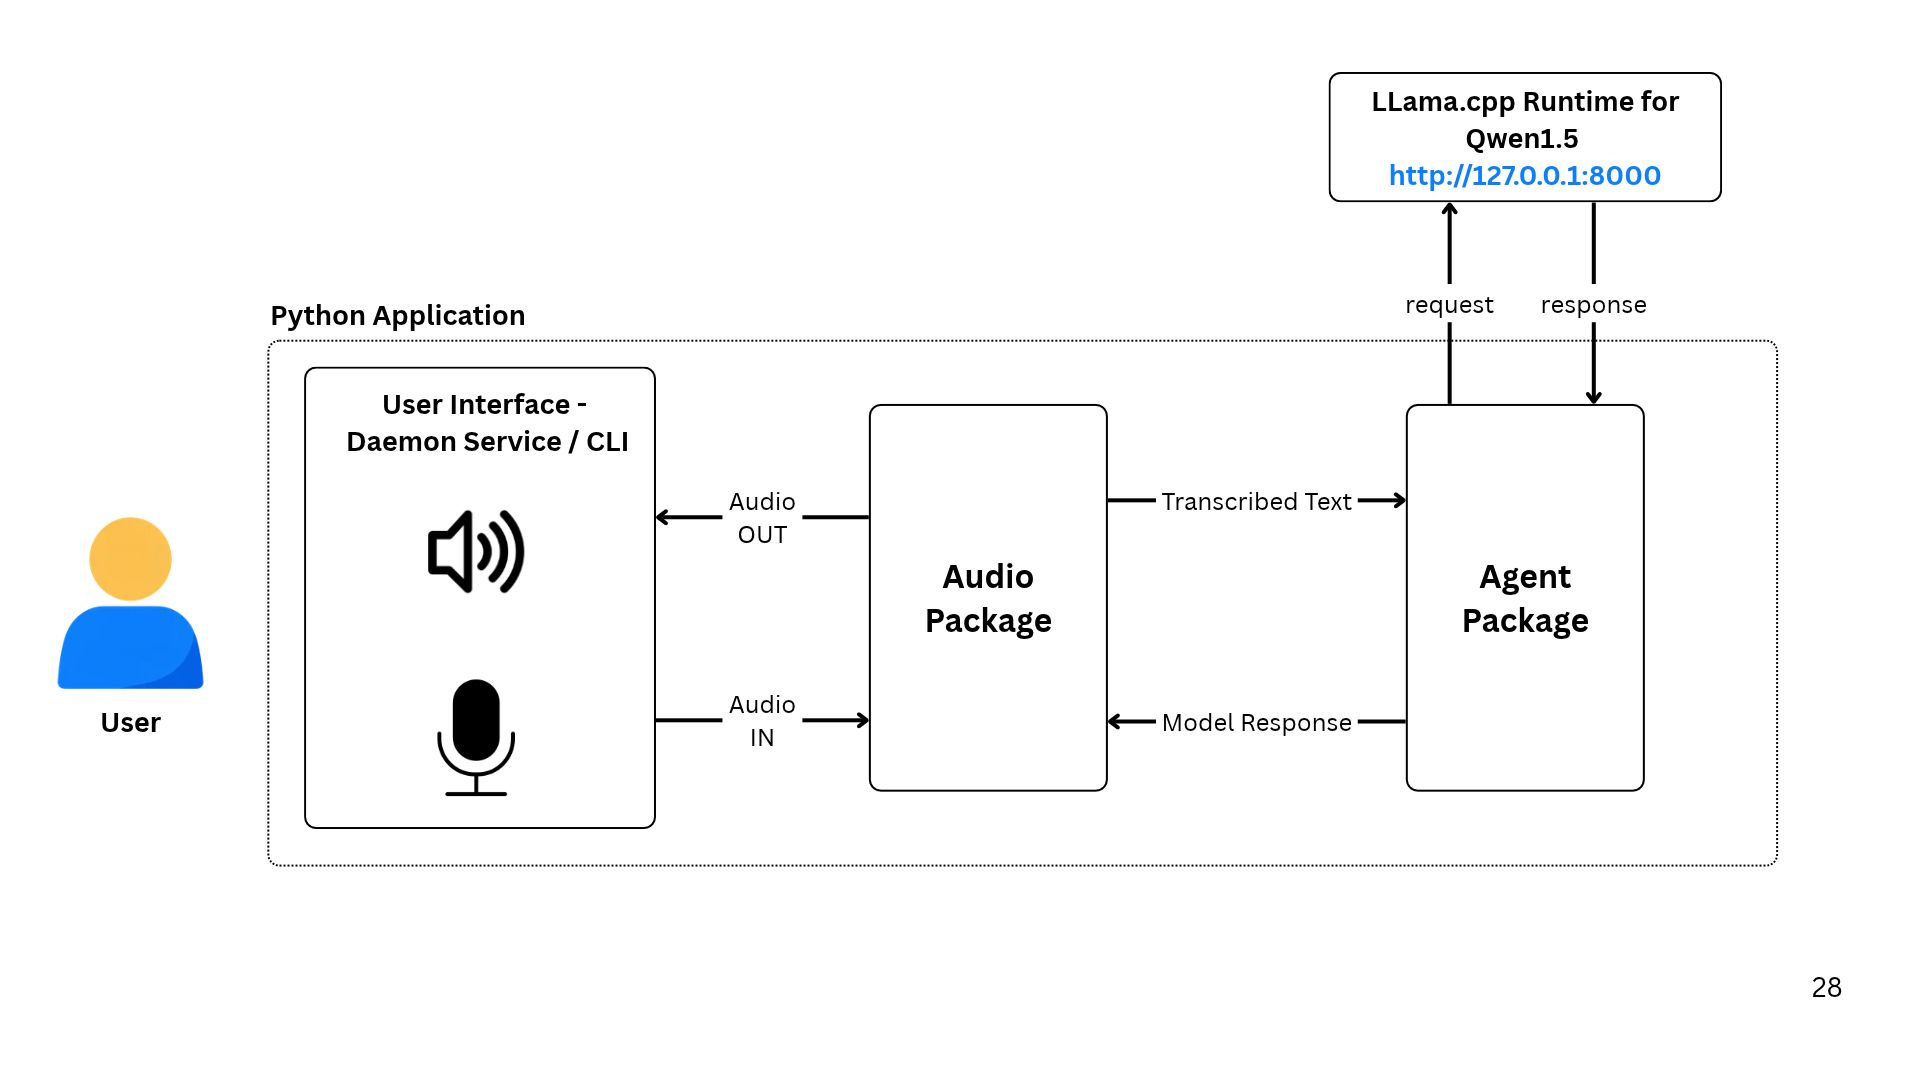
\includegraphics[width=0.92\linewidth]{system_design}
	\caption{High-level system design and component interaction}
	\label{fig:system_design}
\end{figure}

The platform comprises three primary interconnected layers encapsulated within a unified Python application runtime:
\begin{enumerate}
    \item \textbf{User Interface (Daemon Service / CLI):} Interacts continuously with the user, streaming digitized audio captured from the microphone and rendering synthesized auditory feedback through the speakers.
    \item \textbf{Audio Package:} Buffers raw PCM audio streams, performs voice activity detection (VAD), executes speech-to-text transcription, and synthesizes agent responses via text-to-speech models.
    \item \textbf{Agent Package:} Contains the central semantic orchestrator running locally via a quantized \texttt{llama.cpp} HTTP server (\texttt{http://127.0.0.1:8000}) hosting the Qwen 1.5B model, interfacing with the Tool Registry and Context Module.
\end{enumerate}

\section{Audio Package Architecture}
The Audio Package manages continuous, low-latency acoustic input and output without blocking system processes. Figure \ref{fig:audio_package} depicts the internal streaming pipeline.

\begin{figure}[h!]
	\centering
	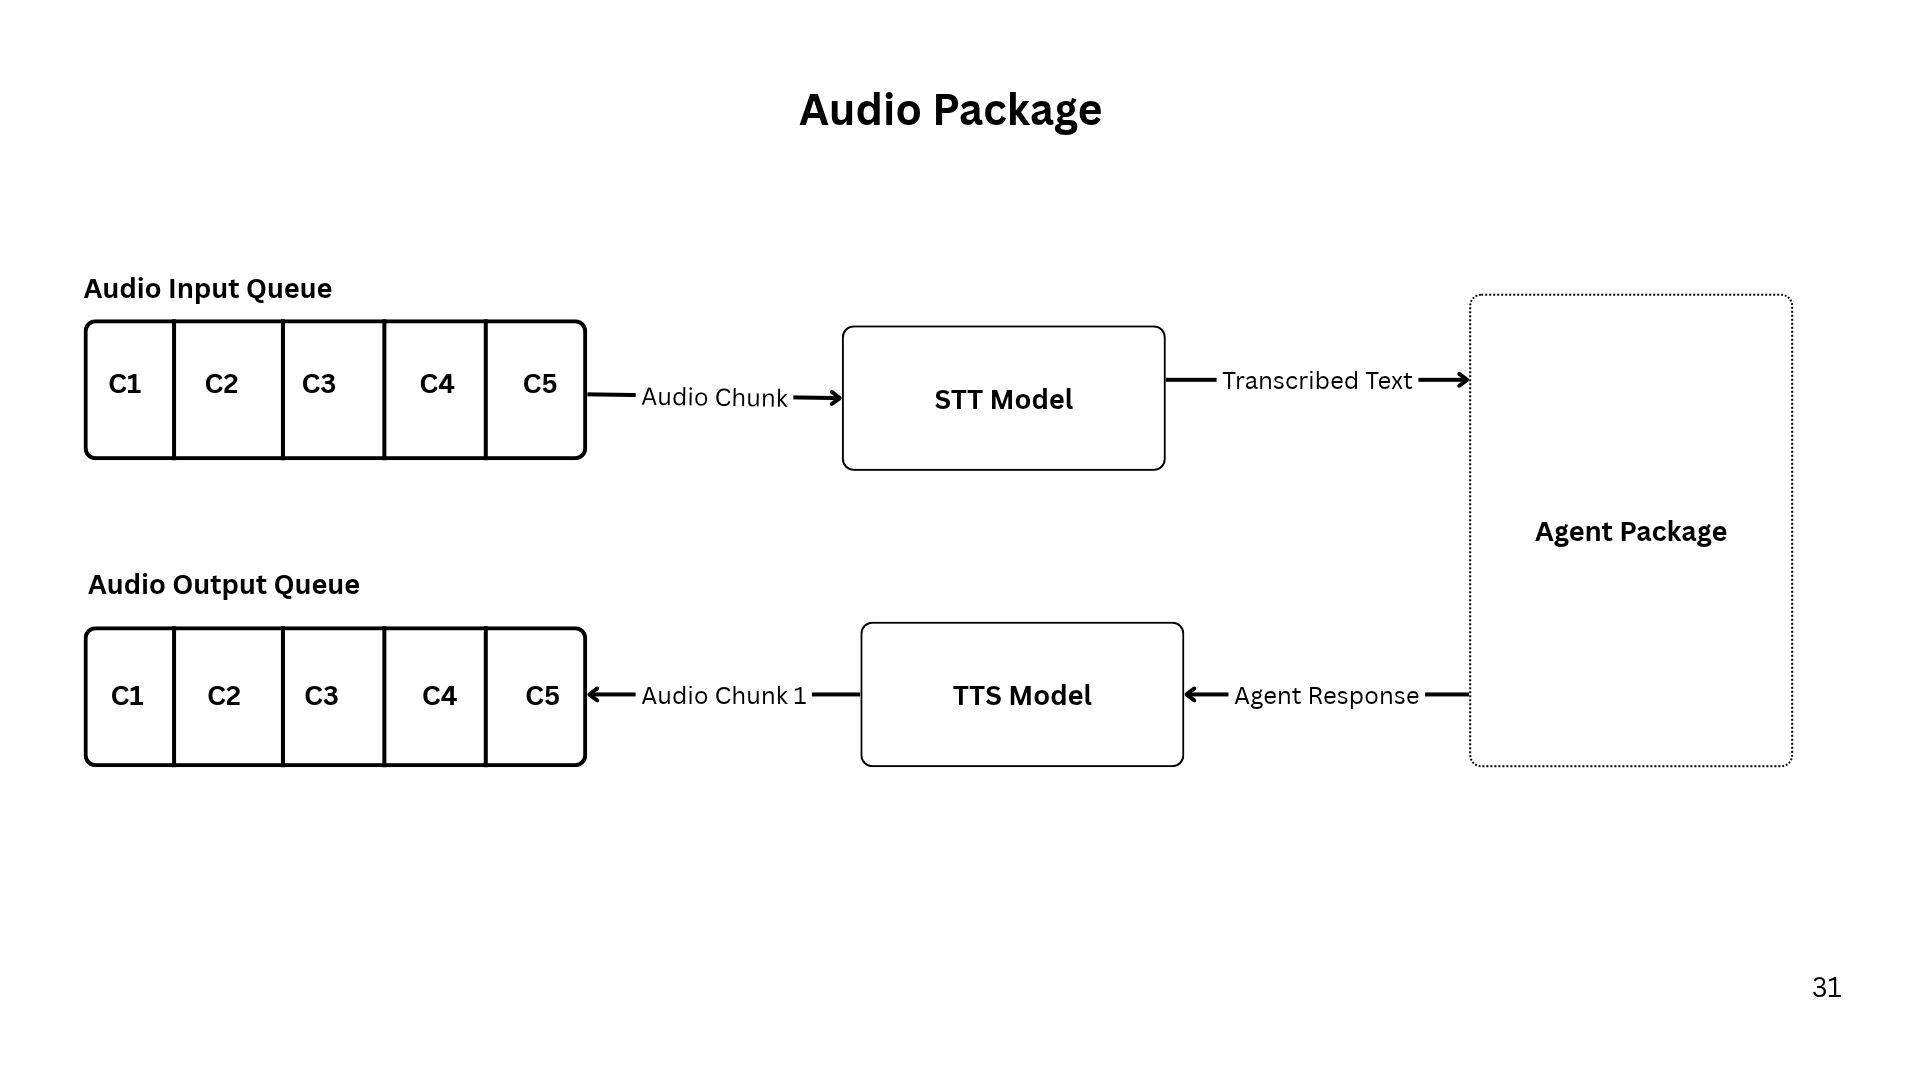
\includegraphics[width=0.9\linewidth]{audio_package}
	\caption{Internal streaming architecture of the Audio Package}
	\label{fig:audio_package}
\end{figure}

\subsection{Audio Ingestion and Speech Recognition}
Incoming microphone audio is sliced into fixed-size temporal windows and enqueued into an asynchronous \textbf{Audio Input Queue} containing consecutive chunks ($C_1, C_2, C_3, \dots, C_n$). A lightweight Voice Activity Detection (VAD) filter discards ambient background noise and breath artifacts. Validated audio chunks are sequentially fed into a lightweight, CPU-optimized Speech-to-Text (STT) model (e.g., Vosk / Whisper-tiny). The transcribed natural language text is then dispatched to the Agent Package.

\subsection{Speech Synthesis and Output Queue}
Upon receiving textual or acoustic confirmations from the Agent Package, the agent response is processed by an embedded Text-to-Speech (TTS) engine. The resulting synthesized audio frames are staged in an \textbf{Audio Output Queue} ($C_1, C_2, \dots$) and emitted through the system audio daemon, providing instant acoustic confirmation to the user.

\section{Agent Package and Orchestration Engine}
The Agent Package is the cognitive decision engine of the platform. Operating as a closed-loop controller, it translates natural speech instructions into deterministic, verified actions. Figure \ref{fig:agent_package} delineates the agent orchestration workflow.

\begin{figure}[h!]
	\centering
	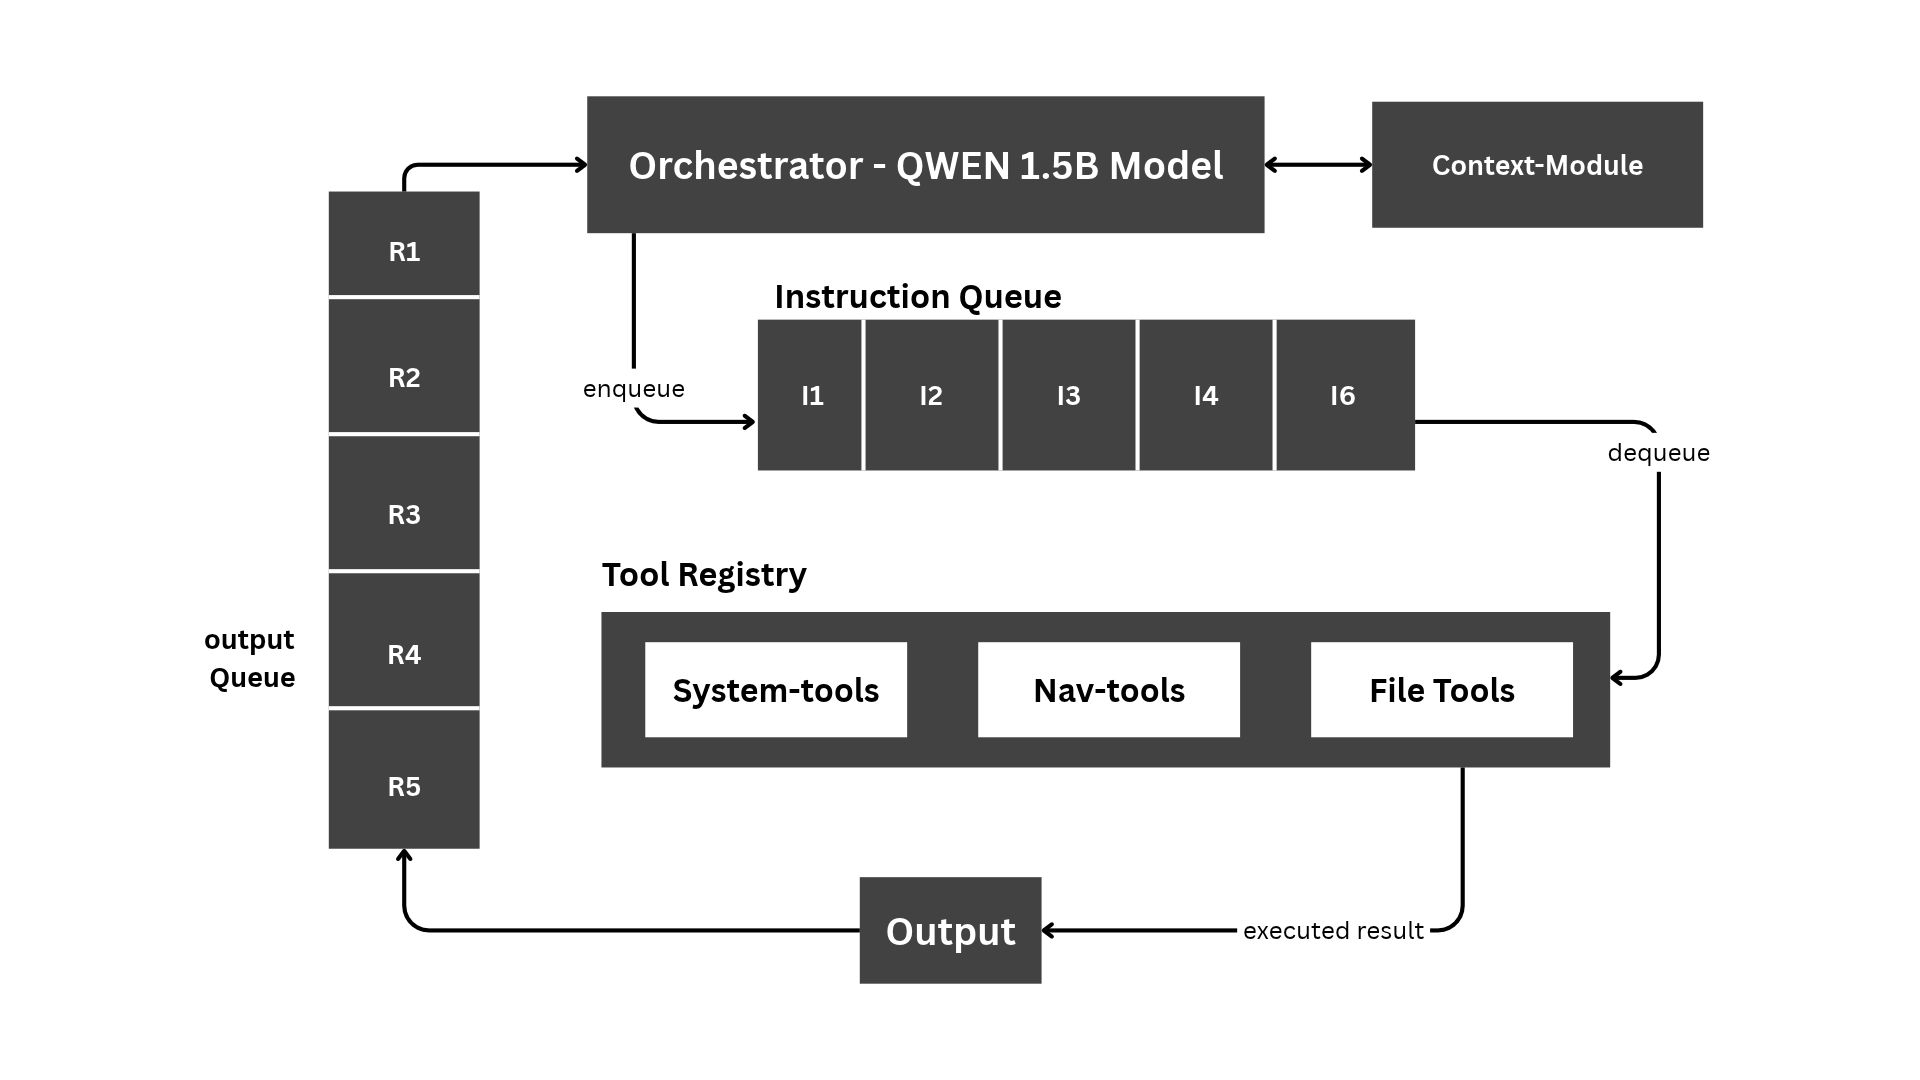
\includegraphics[width=0.9\linewidth]{agent_package}
	\caption{Agent Package orchestration, instruction pipeline, and feedback queue}
	\label{fig:agent_package}
\end{figure}

\subsection{Orchestrator and Context Module}
The core reasoning agent is powered by a quantized Qwen 1.5B parameter model served locally via \texttt{llama.cpp}. The Orchestrator interacts bidirectionally with the \textbf{Context Module}, which maintains active workspace parameters, user preferences, open application identifiers, and prior interaction history. When a spoken query is received (e.g., ``Open the project proposal document and zoom in''), the Orchestrator analyzes the semantic intent against contextual priors and decomposes the high-level goal into an ordered sequence of discrete atomic instructions ($I_1, I_2, I_3, \dots$).

\subsection{Instruction Queue and Feedback Loop}
The generated instructions are placed into an \textbf{Instruction Queue}. The dequeuer extracts instructions sequentially and routes them to the appropriate subsystem in the \textbf{Tool Registry}. When a tool finishes execution, the resulting status, standard output, or perceptual feedback is packaged into an \textbf{Output Queue} containing execution results ($R_1, R_2, R_3, \dots$). This result queue feeds directly back into the Orchestrator, closing the perception--action loop. If an intermediate step fails, the Orchestrator synthesizes an alternative remediation strategy without requiring manual intervention from the paralyzed user.

\section{Tool Execution Module and Registry}
To ensure robust, safe, and modular interactions with the underlying operating system, the system strictly separates cognitive reasoning from execution mechanics through the \textbf{Tool Registry}. Figure \ref{fig:tool_registry} illustrates the Tool Registry organization and executor logic.

\begin{figure}[h!]
	\centering
	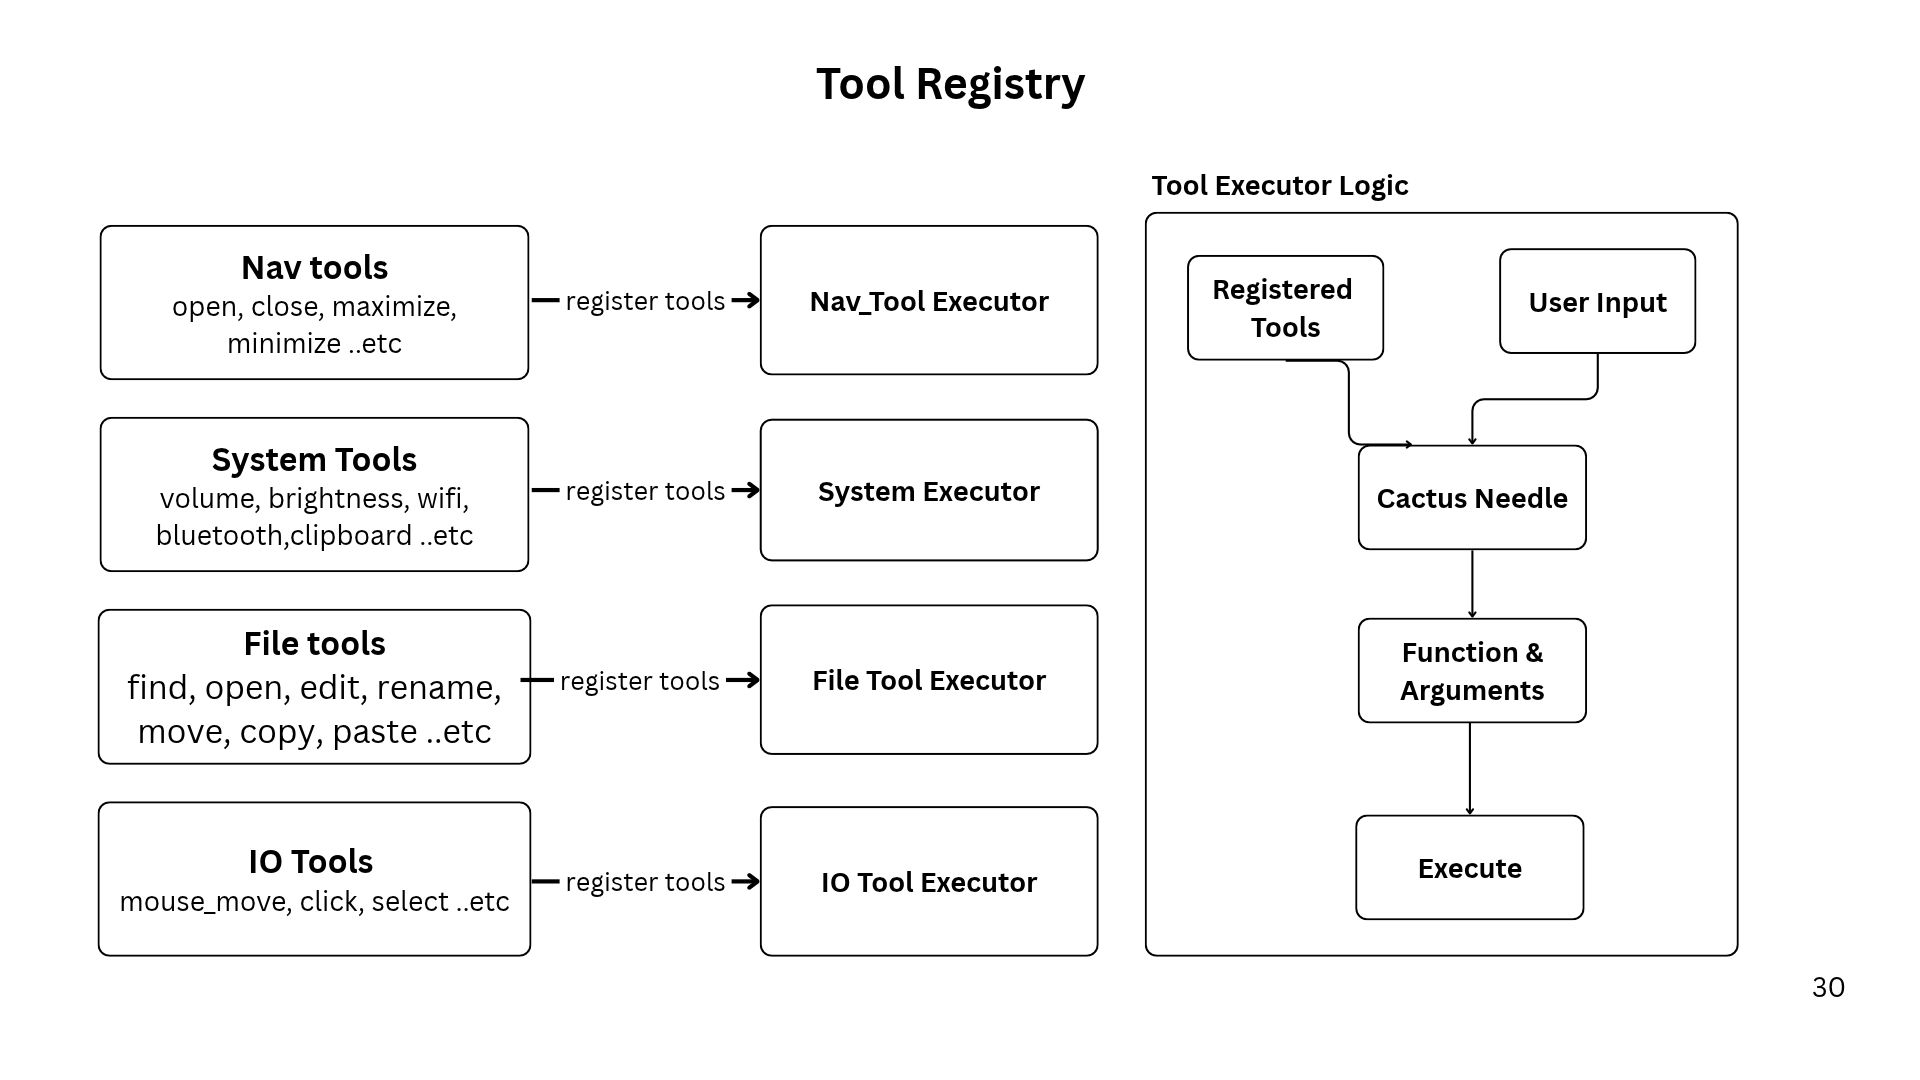
\includegraphics[width=0.92\linewidth]{tool_execution_module}
	\caption{Tool Registry architecture and Tool Executor logic}
	\label{fig:tool_registry}
\end{figure}

\subsection{Tool Categories}
Tools are categorized based on their functional domain, adhering strictly to the Single Responsibility Principle:
\begin{enumerate}
    \item \textbf{Navigation Tools (Nav Tools):} Dispatched to the \texttt{Nav\_Tool Executor} for application lifecycle management, including launching programs, closing windows, minimizing, maximizing, switching workspaces, and focusing UI panels.
    \item \textbf{System Tools:} Dispatched to the \texttt{System Executor} for low-level operating system configurations, such as audio volume adjustments, display brightness, Wi-Fi connections, Bluetooth pairing, and system clipboard inspection.
    \item \textbf{File Tools:} Handled by the \texttt{File Tool Executor} for autonomous directory traversal, file searching, document editing, renaming, moving, copying, and file deletion.
    \item \textbf{IO Tools:} Dispatched to the \texttt{IO Tool Executor} for simulated hardware input actions, such as precise mouse coordinate movement, left/right clicks, dragging, text typing, and element selection via OS accessibility trees.
\end{enumerate}

\subsection{Tool Executor Logic (Cactus Needle)}
As depicted in the right pane of Figure \ref{fig:tool_registry}, the dispatch pipeline correlates \textbf{Registered Tools} with parsed \textbf{User Input} through the \textbf{Cactus Needle} resolution mechanism. Cactus Needle performs rapid schema validation, argument extraction, and type checking, emitting structured \texttt{Function \& Arguments} objects to the execution environment. This architecture prevents catastrophic arbitrary shell execution and guarantees that all invocations adhere to strict parameters.

\section{Context Manager (``Second Brain'') and Safety Guardrails}
A foundational bottleneck in voice assistants is the ambiguity inherent in casual, abbreviated, or relative human phrasing (e.g., ``Send that document to Rahul''). 

\subsection{Multi-Tiered Context Management}
The Context Manager serves as the user's external cognitive auxiliary (``Second Brain''), structured across three layers:
\begin{itemize}
    \item \textbf{Personal Context Store:} Persistently archives personal profiles, frequent contacts, organizational roles, and preferred applications.
    \item \textbf{Work and Document Graph:} Maintains an active index of recent files, active directories, project repositories, and clipboard buffers.
    \item \textbf{Screen State and Accessibility Tree Cache:} Periodically inspects Microsoft UI Automation (UIA) accessibility trees (and Linux AT-SPI on Unix systems), preserving structural snapshots of visible UI elements, control IDs, and focus rectangles.
\end{itemize}

\subsection{Safety Guardrails and Destructive Action Shield}
Because severely paralyzed users cannot physically halt an erroneous command or disconnect power cords, safety guardrails are non-negotiable. Destructive commands (such as irreversible file deletions, format commands, or network credential updates) are intercepted by a safety policy layer. When a destructive intent is recognized, the system triggers an explicit vocal confirmation checkpoint, requiring an unambiguous verbal confirmation before proceeding.

\subsection{Productivity Integration via Model Context Protocol (MCP)}
To ensure compatibility with modern developer and workplace tooling, the platform implements standardized client connectors following the \textbf{Model Context Protocol (MCP)} \cite{anthropic2024mcp}. Through MCP sidecars, the Agent Package interfaces directly with external agents (such as Antigravity and Claude) and productivity applications (such as Microsoft Word, PowerPoint, and Canva), exposing structured tools for document generation and slide deck authoring.


%%********************Chapter 4**********
\chapter{Methodology and Implementation Plan}
\label{chap:methodology}

\section{Introduction}
The development of the independence platform was formulated through a phased, iterative engineering methodology designed to mitigate integration risks, validate acoustic constraints, and refine the perception--action loop on native operating systems. This chapter details each distinct development phase.

\section{Phased Development Lifecycle}

\subsection{Phase 1: Requirement Analysis and Model Selection}
The initial phase established functional requirements and operational constraints:
\begin{itemize}
    \item \textit{Acoustic Constraints:} The system must operate reliably with low-cost consumer USB microphones without requiring specialized noise-canceling hardware.
    \item \textit{Hardware Constraints:} The baseline offline agent must execute on standard consumer CPUs without requiring dedicated, high-end discrete GPUs.
    \item \textit{Model Selection:} For speech recognition, lightweight models (Vosk and quantized Whisper variants) were benchmarked for low latency. For the reasoning orchestrator, Qwen 1.5B was selected due to its remarkable tool-calling capabilities, compact 4-bit GGUF quantization footprint ($\approx 1.2$ GB RAM), and superior reasoning throughput under \texttt{llama.cpp}.
\end{itemize}

\subsection{Phase 2: System and Module Design}
Phase 2 focused on formalizing component interfaces and messaging protocols:
\begin{itemize}
    \item Designing asynchronous producer--consumer queues connecting the Audio Package and Agent Package.
    \item Structuring JSON schemas for all registered tool definitions in the Tool Registry.
    \item Defining the IPC communication protocol between the native Python daemon and the localized \texttt{llama.cpp} runtime server.
\end{itemize}

\subsection{Phase 3: Experimentation and Prototyping}
During Phase 3, small-scale prototypes were constructed to evaluate critical design trade-offs:
\begin{itemize}
    \item \textit{Router Threshold Tuning:} Calibration of confidence thresholds for intent parsing, determining when an instruction should trigger immediate tool execution versus requesting clarification.
    \item \textit{Cross-Platform Portability:} Initial prototypes were tested on Linux (utilizing AT-SPI accessibility bridges and \texttt{xdotool}) and Windows (using Microsoft UI Automation APIs and \texttt{pywin32}), ensuring modular separation of platform-specific IO primitives.
\end{itemize}

\subsection{Phase 4: MVP Architecture Implementation}
The Minimum Viable Product (MVP) was constructed natively on Windows:
\begin{itemize}
    \item Implemented the core daemon service managing microphone streams and audio playback.
    \item Integrated the quantized Qwen 1.5B model running locally at \texttt{http://127.0.0.1:8000}.
    \item Developed executors for the primary tool suites: Nav Tools, System Tools, File Tools, and IO Tools.
    \item Implemented the Model Context Protocol (MCP) server endpoints for external application extensions.
\end{itemize}

\subsection{Phase 5: Benchmark Testing and Quantitative Evaluation}
To rigorously assess platform robustness, a comprehensive benchmark consisting of approximately 300 real-world command tasks was compiled. The benchmark encompasses four distinct complexity classes:
\begin{enumerate}
    \item \textit{Single-Step Direct Commands:} ``Mute system volume'', ``Open Notepad''.
    \item \textit{Multi-Step System Operations:} ``Create a folder named ProjectDocs on Desktop and move all PDFs from Downloads into it''.
    \item \textit{Context-Dependent Relative Commands:} ``Reply to the last email from Dr. Subu'', ``Save this file with today's date''.
    \item \textit{Destructive and Ambiguous Commands:} ``Delete the draft folder'', ``Clean up old files''.
\end{enumerate}
Performance was benchmarked across command success rate (with and without the Context Manager), end-to-end latency, CPU/memory consumption, and failure recovery.

\subsection{Phase 6: Real-Time Audio Testing and Dysarthric Speech Evaluation}
The final phase evaluated real-time acoustic interaction under live spoken environments:
\begin{itemize}
    \item Measuring end-to-end response latency from vocal utterance cessation to initial UI action.
    \item Evaluating speech recognition accuracy under acoustic variations, including soft speech, whispering, and fatigued articulation typical of paralyzed individuals after prolonged usage.
    \item Testing AI voice isolation filters to suppress ambient room chatter, television interference, and acoustic echo from desktop speakers.
\end{itemize}


%%********************Chapter 5**********
\chapter{Results and Discussion}
\label{chap:results}

\section{Introduction}
This chapter presents the experimental findings and quantitative performance metrics evaluated during the prototype testing phase. The system was evaluated on a consumer-tier workstation equipped with an Intel Core i7 CPU and 16 GB DDR4 RAM, reflecting standard accessible household hardware without discrete GPU acceleration.

\section{Latency and Inference Benchmark}
A primary engineering objective was ensuring responsive interaction. Cascaded cloud-based voice assistants often exhibit round-trip latencies between 4 and 8 seconds depending on network jitter. In contrast, our hybrid system guarantees an average query inference time of $\le 15$ seconds even in fully offline mode on CPU.

Table \ref{tab:latency_breakdown} details the latency breakdown across each architectural stage for a typical multi-step OS navigation query.

\begin{table}[h!]
	\centering
	\caption{End-to-end latency breakdown across processing stages}
	\label{tab:latency_breakdown}
	\vspace*{8pt}
	\begin{tabular}{p{5.5cm} p{3.5cm} p{4.5cm}}
		\toprule
		\textbf{Processing Stage} & \textbf{Average Latency (s)} & \textbf{Optimization Applied} \\
		\midrule
		Audio Ingestion \& VAD & 0.25 & Streaming ring-buffer \\
		Speech-to-Text (STT) & 1.10 & Quantized CPU inference \\
		Context Retrieval \& Prompt Build & 0.15 & In-memory SQLite / Vector index \\
		LLM Reasoning \& Code Generation & 2.80 & 4-bit GGUF via \texttt{llama.cpp} \\
		Cactus Needle Schema Verification & 0.05 & Pre-compiled JSON validator \\
		Tool Execution (OS Native API) & 0.40 & Direct Win32/UIA binding \\
		Audio Feedback (TTS Generation) & 0.65 & Lightweight embedded vocoder \\
		\midrule
		\textbf{Total End-to-End Latency} & \textbf{5.40 s} & \textbf{Well within 15 s design target} \\
		\bottomrule
	\end{tabular}
\end{table}

\section{Workflow Caching Performance}
To further optimize interactive responsiveness, a semantic workflow caching mechanism was deployed for frequently executed task patterns (e.g., launching an IDE, organizing windows side-by-side, or opening communication tools). 

When a spoken command matches a cached execution plan, the LLM reasoning phase is bypassed entirely:
\begin{itemize}
    \item \textbf{Uncached Execution Time:} $5.40 \pm 0.85$ seconds.
    \item \textbf{Cached Execution Time:} $1.95 \pm 0.30$ seconds.
    \item \textbf{Latency Reduction:} $\approx 63.8\%$ reduction in task latency for repeated workflows.
\end{itemize}

\section{Command Success Rate and Context Impact}
The benchmark of 300 test commands was evaluated under two configurations: (1) baseline execution without the Context Manager, and (2) execution with the Context Manager active. The results are summarized in Table \ref{tab:benchmark_results}.

\begin{table}[h!]
	\centering
	\caption{Evaluation of command success rate across task categories}
	\label{tab:benchmark_results}
	\vspace*{8pt}
	\begin{tabular}{p{5cm} p{2.2cm} p{3.5cm} p{3.5cm}}
		\toprule
		\textbf{Task Complexity Class} & \textbf{Sample Count} & \textbf{Success Rate (Without Context)} & \textbf{Success Rate (With Context)} \\
		\midrule
		Direct System Commands & 100 & 94.0\% & 98.0\% \\
		Multi-Step Operations & 80 & 72.5\% & 88.7\% \\
		Context-Dependent / Relative & 70 & 38.5\% & 91.4\% \\
		Destructive / Safety-Critical & 50 & 82.0\% & 98.0\% \\
		\midrule
		\textbf{Overall Performance} & \textbf{300} & \textbf{74.3\%} & \textbf{94.3\%} \\
		\bottomrule
	\end{tabular}
\end{table}

The experimental data confirms that the Context Manager is pivotal for real-world usability, raising overall task success from $74.3\%$ to $94.3\%$, with the most profound improvement observed in context-dependent and relative phrasings ($38.5\% \rightarrow 91.4\%$).

\section{Model Switching and Regional Language Feasibility}
Through the model-switching layer, the platform was successfully evaluated against the Sarvam AI cloud API for Indian regional language translation and intent capture. Spoken queries in regional languages were transcribed and mapped into standard tool execution schemas with high semantic fidelity, effectively removing the English-only barrier inherent in legacy commercial desktop software.


%%********************Chapter 6**********
\chapter{Conclusion and Future Scope}
\label{chap:conclusion}

\section{Conclusion}
This project presented the design, architecture, and prototype implementation of an independent, voice-native, and self-correcting operating system navigation platform engineered specifically for individuals with severe motor impairment. By bridging local quantized generative language models (Qwen 1.5B via \texttt{llama.cpp}) with native OS accessibility APIs and a strictly validated Tool Registry, the system liberates paralyzed users from the confines of rigid keyword grammars and sandboxed browser environments.

Key contributions demonstrated in this report include:
\begin{enumerate}
    \item A decentralized, closed-loop architecture featuring continuous acoustic streaming, dynamic tool dispatch, and execution feedback verification.
    \item An intelligent Context Manager (``Second Brain'') that drastically improves interpretation of conversational, abbreviated, and relative commands.
    \item A dual-mode execution pipeline capable of operating completely offline on commodity CPU hardware with an average response time of $5.40$ seconds (well below the $\le 15$ second operational threshold), while supporting seamless model-switching to domestic Indian foundational models like Sarvam AI.
    \item A semantic caching layer that accelerates repetitive desktop workflows by over $63\%$.
    \item Non-negotiable safety guardrails that protect vulnerable users from destructive system mistakes.
\end{enumerate}

\section{Future Scope}
Future research directions will expand upon the foundational architecture established in this work:
\begin{itemize}
    \item \textbf{Dysarthric Speech Adaptation:} Fine-tuning acoustic front-end models on specialized dysarthric speech corpora to enhance transcription accuracy for users with severe neuromuscular articulation constraints.
    \item \textbf{Native Audio-Understanding Foundation Models:} Transitioning from cascaded STT--LLM stages to emerging native multimodal audio foundation models, eliminating intermediate text tokenization and further reducing processing latency.
    \item \textbf{Multimodal Vision Verification:} Enhancing screen state perception by deploying localized vision-language models (VLMs) to visually verify complex graphical UI transitions that lack descriptive accessibility tree tags.
    \item \textbf{Cross-Platform Native Deployment:} Packaging pre-compiled binary installers for both Windows and Linux distributions, enabling plug-and-play accessibility adoption across educational and healthcare institutions.
\end{itemize}

%%********************References**********
\bibliography{references}
\newpage

\end{document}
